Die Highlevel Steuerung besteht aus einer Komponenten \glqq cup\textunderscore acceptor\textunderscore manager\grqq, die sowohl die Koordination der Teile innerhalb der Gruppe, als auch die Kommunikation mit dem Super Manager koordiniert. Dazu stellte diese Komponente eine Action mit dem Namen AcceptCup zur Verfügung, die nach einer erfolgreichen Bilderkennung die Tasse greift und auf den Turtlebot stellt. Der Aktivitätenfluss gestaltet sich wie folgt:
\begin{enumerate}
\item Abonnement auf Ergebnisse der Localization Komponente
\item AcceptCup Action wird aufgerufen
\item Überprüfe Bounding Boxes für Tasse und Turtlebot. Ohne Ergebnisse wird gewartet und Fortschritt gemeldet
\item Aufrufen der Gripper Arm Action

\item Feedback zurückgeben
\end{enumerate}

Der besondere Augenmerk lag auf einer korrekten Implementierung der Schnittstellen zu den anderen Gruppen.

\begin{figure}
\centering
\begin{minipage}[t]{.5\textwidth}
\centering
\vspace{0pt}
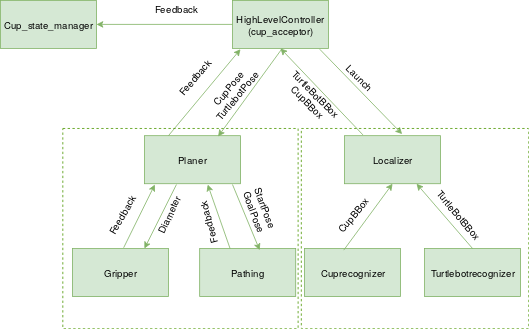
\includegraphics[width=10cm]{./images/highlevel_Diagram.png}
\caption{Diagram des Highlevel-Controls}
\end{minipage}\hfill
\begin{minipage}[t]{.3\textwidth}

\hfill

\centering
\vspace{0pt}
\begin{tabular}{ |c|c| }
 \hline
 Code & Feedback \\ 
 \hline
 200 & success \\ 
 301 & cup not reachable \\ 
 302 & turtlebot not reachable \\
 401 & cup not found \\
 402 & turtlebot not found \\
 500 & path planing failed \\
 600 & unknown \\ 
 \hline
\end{tabular}\\
 \captionof{table}{Feedback tabelle}
\end{minipage}
\end{figure}

Der besondere Augenmerk lag auf einer korrekten Implementierung der Schnittstellen zu den anderen Gruppen.
